\documentclass{standalone}
\usepackage[T1]{fontenc}
\usepackage[latin2]{inputenc}
\usepackage[english]{babel}
\usepackage{tikz}
\usepackage{times}
\usetikzlibrary{calc,through,backgrounds,positioning,fit}
\usetikzlibrary{shapes,arrows,shadows,calendar}
\begin{document}

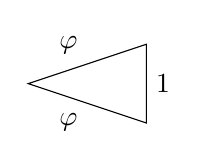
\begin{tikzpicture}
\draw (0,0) -- (1.5,0.5)node[midway, above left]{$\varphi$} --(1.5,-0.5) node[midway,right]{$1$}--cycle node[midway, below left]{$\varphi$};
\end{tikzpicture}
\end{document}